\documentclass[a4paper,11pt]{article}

\usepackage[utf8]{inputenc}%para caracteres especiales
\usepackage{color}
\usepackage{array}
\usepackage[Spanish]{babel}%idioma
\usepackage{amsmath,amssymb}
\usepackage{graphicx}%para incluir graficos
\usepackage{ragged2e}
\usepackage[colorlinks,linkcolor=black]{hyperref}%para hacer hipervinculos
\usepackage{multicol}%para generar columnas
\usepackage{algpseudocode}%para pseudocodigo
\usepackage{float}
\usepackage{subfig}
\usepackage{enumerate}


\addtolength{\textwidth}{2cm}
\addtolength{\hoffset}{-1cm}





\begin{document}

\setlength{\topmargin}{-0,2in}
%caratula


\vspace*{\fill}
			\begin{center}
				\textbf{
					\vspace{-0.7em}
					ESCUELA SUPERIOR POLITÉCNICA DEL LITORAL
				}
				\line(1,0){380}\\		
				\scriptsize{FACULTAD DE INGENIERÍA EN ELECTRICIDAD Y COMPUTACIÓN}
				
				\vspace{2.5em}
				
\includegraphics[scale=0.5]{image_buscamina/espol.jpg} 
			\end{center}
			
			\begin{center}
				\vspace{2.5em}
				Lenguajes de Programación
				\\II Término - 2013\\
				\vspace{3.5em}  %espacio entre linea anterior y la siguiente
				\textbf{"Proyecto Primer Parcial''}
				\vspace{5em}
			\end{center}	

\vspace*{\fill}
\newpage 

\tableofcontents

\newpage


\vspace*{\fill}
\textbf{Proyecto Buscamina en Android}
\vspace{5em}
\begin{center}
	
\includegraphics[scale=0.5]{image_buscamina/android.jpg} 
\end{center}
	
\vspace*{\fill}


\newpage 
	
\vspace*{\fill}
\begin{center}
		
                        
\includegraphics[scale=1.5]{image_buscamina/papel_hueco.jpg} 
	\end{center}
	
			\begin{center}
				Manual de Usuario \\
				\vspace{5em}
				\Huge{\textbf{``Buscamina''	\vspace{3em}}}
			\end{center}	
			
			


				\hspace*{5cm}Desarrolladores:
				\vspace{1.5em}
				\\\hspace*{8cm}Jonathan Mendieta
				\\\hspace*{8cm}Dennise Pintado
				\\\hspace*{8cm}Janina Costa


\vspace*{\fill}
\newpage 


\section{Introducción}
El juego a implementar es el buscamina, con tres niveles de juego facil, intermedio y difícil. El lenguaje en el que se debe programar  es Android y nosotros hemos utilizado eclipse como IDE de desarrollo. La implementación del juego se ha basado en una serie de layout tomando diferentes tipos para cada pantalla que creemos. El programar en Android representa un reto se ha buscado destacar la cualidad más grande del lenguaje que es sus graficos. Las aplicaciones dirigidas a dispositivos móviles o tablets son muy llamativo. Así pues nosotros hemos prestado mucha atención en los graficos e imagenes que utilizaremos ya que este tipo de aplicaciones son muy visuales. Este programa aparte de las dificultades tiene una opción de Records donde se guardará una lista de las personas que han terminado el juego y en que tiempo lo han hecho, también tendrá dos secciones una de informacion acerca del juego y otra donde se hable acerca de los desarrolladores. Estas son las especificaciones del juego que esperamos  cumplir.



\section{Alcance}

El proyecto permite todas las opciones del buscaminas que ya conocemos. Al iniciar el juego podemos escoger los niveles de dificultad que están agrupados en tres categorías\textbf{ fácil, difícil e intermedio} luego de esto observaremos el tablero de acuerdo a la dificultad escogida donde tendremos dos secciones(layouts) donde tendremos de la izquierdo nuestro cronometro, nuestro emoticón o carita y nuestras banderas. Podemos dar click a la carita si deseamos resetear nuestro juego y solo se nos pedirá el nombre en caso de haber ganado. Al regresar al menú principal tenemos cuatro opciones ya sea la de iniciar un juego que es la mencionada anteriormente, la de records que nos da una lista de los jugadores con sus tiempos, una descripción de los desarrolladores y un poco de información  de como jugar el buscaminas.
Como limitaciones del juego tenemos el zoom algo que no se pudo implementar por falta de tiempo, el juego esta diseñado para tablets solamente y no puede es sensible a rotación del dispositivo automáticamente se coloca en landscape. 

\newpage


\section{Descripción del Juego Buscamina}
Para implementar el juego utilizamos layouts como tablerow, linearlayout y relativelayout. Se ha implementado para la primera pantalla un hilo que dura 4 segundos en los cuales se reproduce una música de fondo, luego de eso tenemos la pantalla menú que nos muestra varias opciones como dificultades del juego , records, desarrolladores y acerca del juego.Cuando tome la opción de desarrolladores se muestra información acerca de los que implementaron el juego, en acerca de se muestra instrucciones del juego y en records una lista que esta guardada mediante una base de datos que nos permite tener una lista de los jugadores que han ganado y en cuanto tiempo lo han hecho. Mas adelante se detallan caracteristicas del juego que fueron importantes para poder cumplir con lo propuesto







\begin{center}

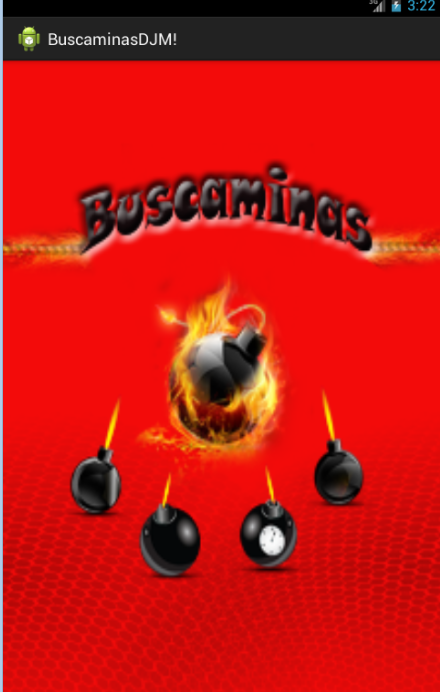
\includegraphics{image_buscamina/pantallaInicial}
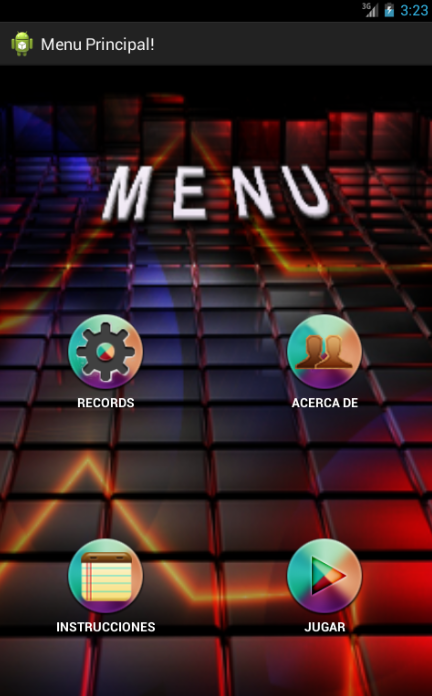
\includegraphics{image_buscamina/pantallaMenu}



\end{center}


Cuando se ingresa a la opción de dificultades se puede escoger entre tres de ellas como facil, intermedio o dificil. Depende de cual se coja se generara un tablero de diferentes dimensiones 9x9 para la primera dificultad, 16x16 para la segunda dificultad y 16x30 para el nivel mas dificil. El tablero esta implementado en un linear layout que tiene un scroll bar para poder visualizar todo el tablero ya que es muy difícil hacer caber todo el tablero en la pantalla porque los cuadrado no se podrían hacer tan pequeños esto no sería bueno para todo tipos de usuarios, por eso se opta determinar un tamaño fijo para las casillas.

\begin{center}

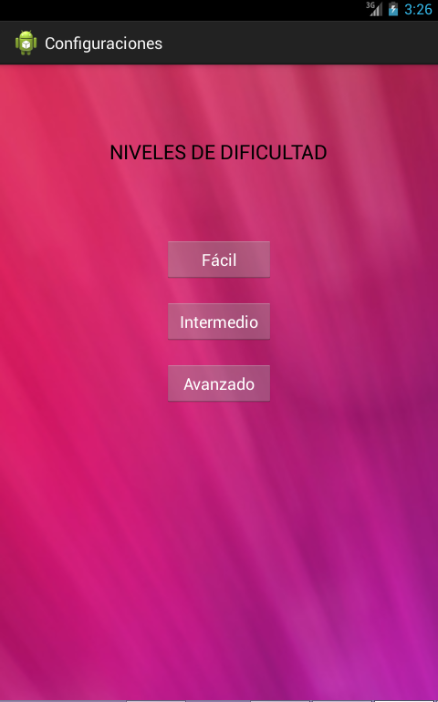
\includegraphics{image_buscamina/dificultades}

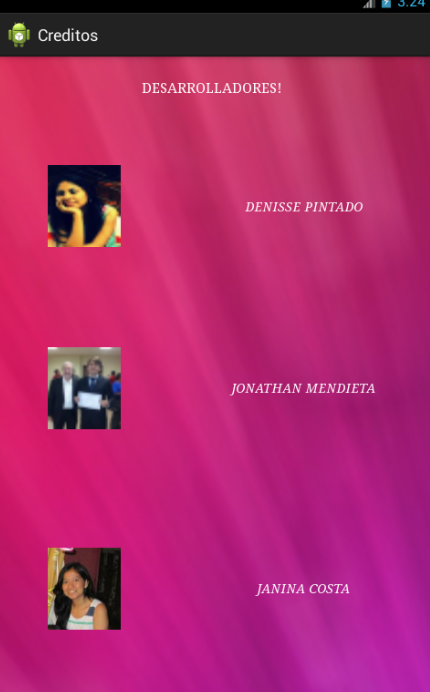
\includegraphics{image_buscamina/pantallaCreditos}

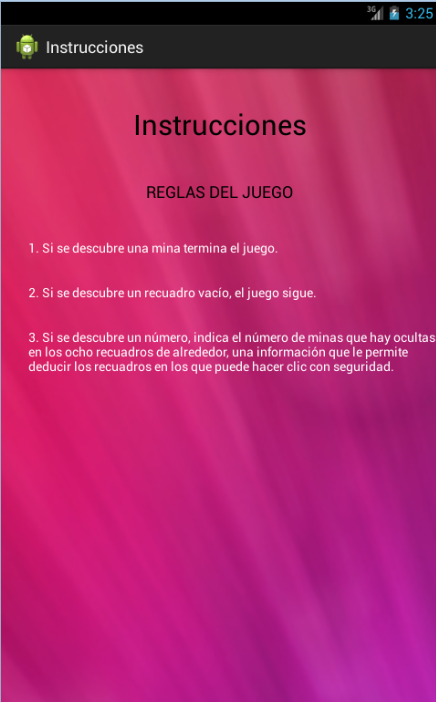
\includegraphics{image_buscamina/pantallaInstrucciones}


\end{center}

Las  diferentes pantallas que se muestran han sido diseñadas con mucha cautela tratando de acertar en el diseño de los juegos tradicionales.Para el juego tenemos la primera pantalla que muestra un cronómetro que nos muestra los segundos de juego,  arriba de el un emoticon que cambia según el estado del jugador en el juego si pierde por una mina la cara cambiara de feliz a triste y si termina el juego bien aparecerá un emoticon de cool.

\begin{center}

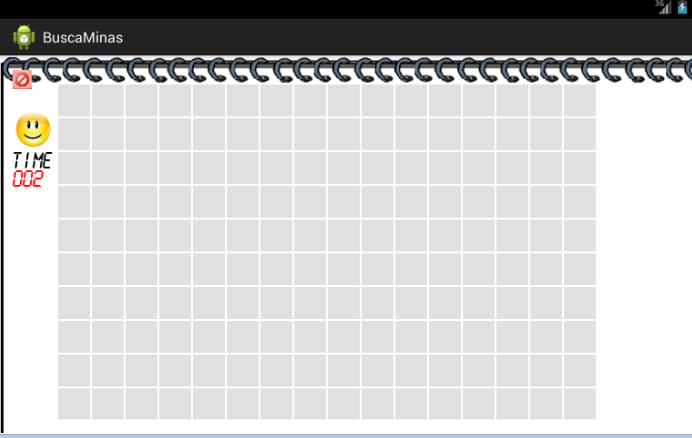
\includegraphics{image_buscamina/pantallaJuegoInicio}

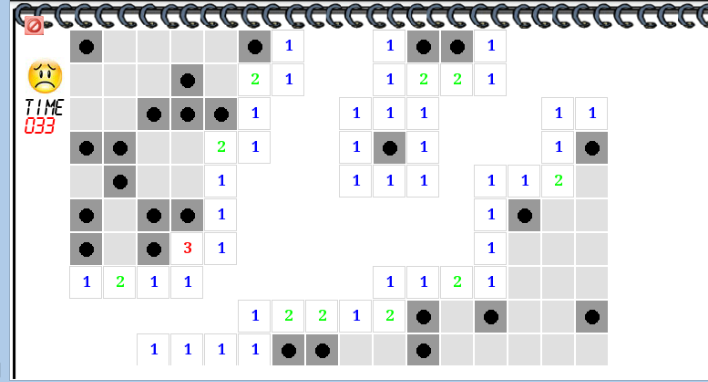
\includegraphics{image_buscamina/pantallaJuego}

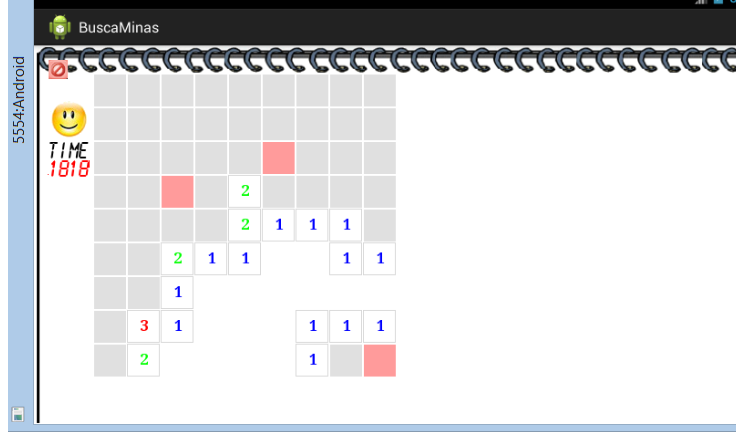
\includegraphics{image_buscamina/banderas}


\end{center}

\section{Bibliografía}

\begin{thebibliography}{99}
\bibitem{layouts}http://maxkalavera.blogspot.com/2012/05/botones-y-listeners-android.html
\bibitem{tableRow}http://developer.android.com/reference/android/widget/TableRow.html
\bibitem{tutoAndroid}https://www.tutos4u.com/android.php?cod=19.-%20Crear%20nueva%20Clase%20(Activity).
\end{thebibliography}

\end{document}